\section{Optimizing the LS$^{2}$ simulation engine}
\label{Implementation}
In the following section I will describe how I optimized the LS$^{2}$ simulation engine using mainly SSE intrinsics. I will begin introducing the software itself and its research purpose. Then, I will document the approach taken for development, including information about how I benchmarked the application in order to acquire meaningful results. The main part of this section will comprise an overview of the optimized source codes of the three algorithms that I have chosen to improve. Code sections of particular interest with regards to special SSE programming techniques will be singled out and explained in detail.
\subsection{LS$^{2}$: A simulation engine for lateration algorithms}

The term "lateration algorithms" is commonly used to refer to geometric algorithms that use distance measurements to determine the location of points in the plane or in a three-dimensional space (as opposed to triangulation which uses the measurement of angles). The most basic representative of this group of algorithms is known as \emph{Trilateration}: Obviously, in the euclidean plane it needs at least three known spots (subsequently called \emph{anchors}) and the distance measurements hereof to be able to narrow down the current position to a single point. Relative to each of the anchors, this point lies on a circle that has its center on the anchor and the distance as its radius. Trilateration determines the current position by solving these three linear equations, in other words, it calculates the intersection of the three circles drawn around the anchors. In real-world applications such as the Global Positioning System (GPS) or indoor localization, distance measurements, like all physically measured data, are generally error-prone. Most commonly, distances are estimated by measuring the time it takes a signal (e.g. light, radio) to travel between an anchor and the client. Because of these erroneous distances, circles drawn around the anchors do not necessarily intersect at a single point and the basic trilateration algorithm fails to produce an exact result. In order to calculate an approximation of the current position, trilateration can be adapted to return the geometric center of the now up to three circle intersections. However, during the last decades, several superior, more complex algorithms have been found that compute improved position estimations based on error-prone distances of three or more anchors.

The \emph{FU Berlin Parallel Lateration-Algorithm Simulation and Visualization Engine} (LS$^{2}$), written by Heiko Will, Thomas Hillebrandt, and Marcel Kyas and first presented at the WPNC conference 2012, is a graphical evaluation framework for lateration algorithms. As the authors explain in~\cite{will2012ls2}, the application's fundamental idea is to not only calculate an average algorithm error based on randomized locations, which has been the main evaluation criterium for lateration algorithms so far, but to calculate errors for all locations on a given "playing field" in parallel and in the end to provide the user with an image displaying the so-called \emph{spatial position error distribution}. The assumption is that the position of the anchors has significant influence on the algorithm's performance, even more so than the errors of the distances. Figure \ref{fig:lateration} shows an exemplary output image created with the LS$^{2}$ engine using the "vble\_opt" algorithm and a set of 3 anchors, only the anchor positions have been slighty magnified for better visibility. The left part of the image displays the average position error for every location (where yellow means low average error), whereas part to the right displays the highest error for every position.

\begin{figure}[h]
\begin{center}
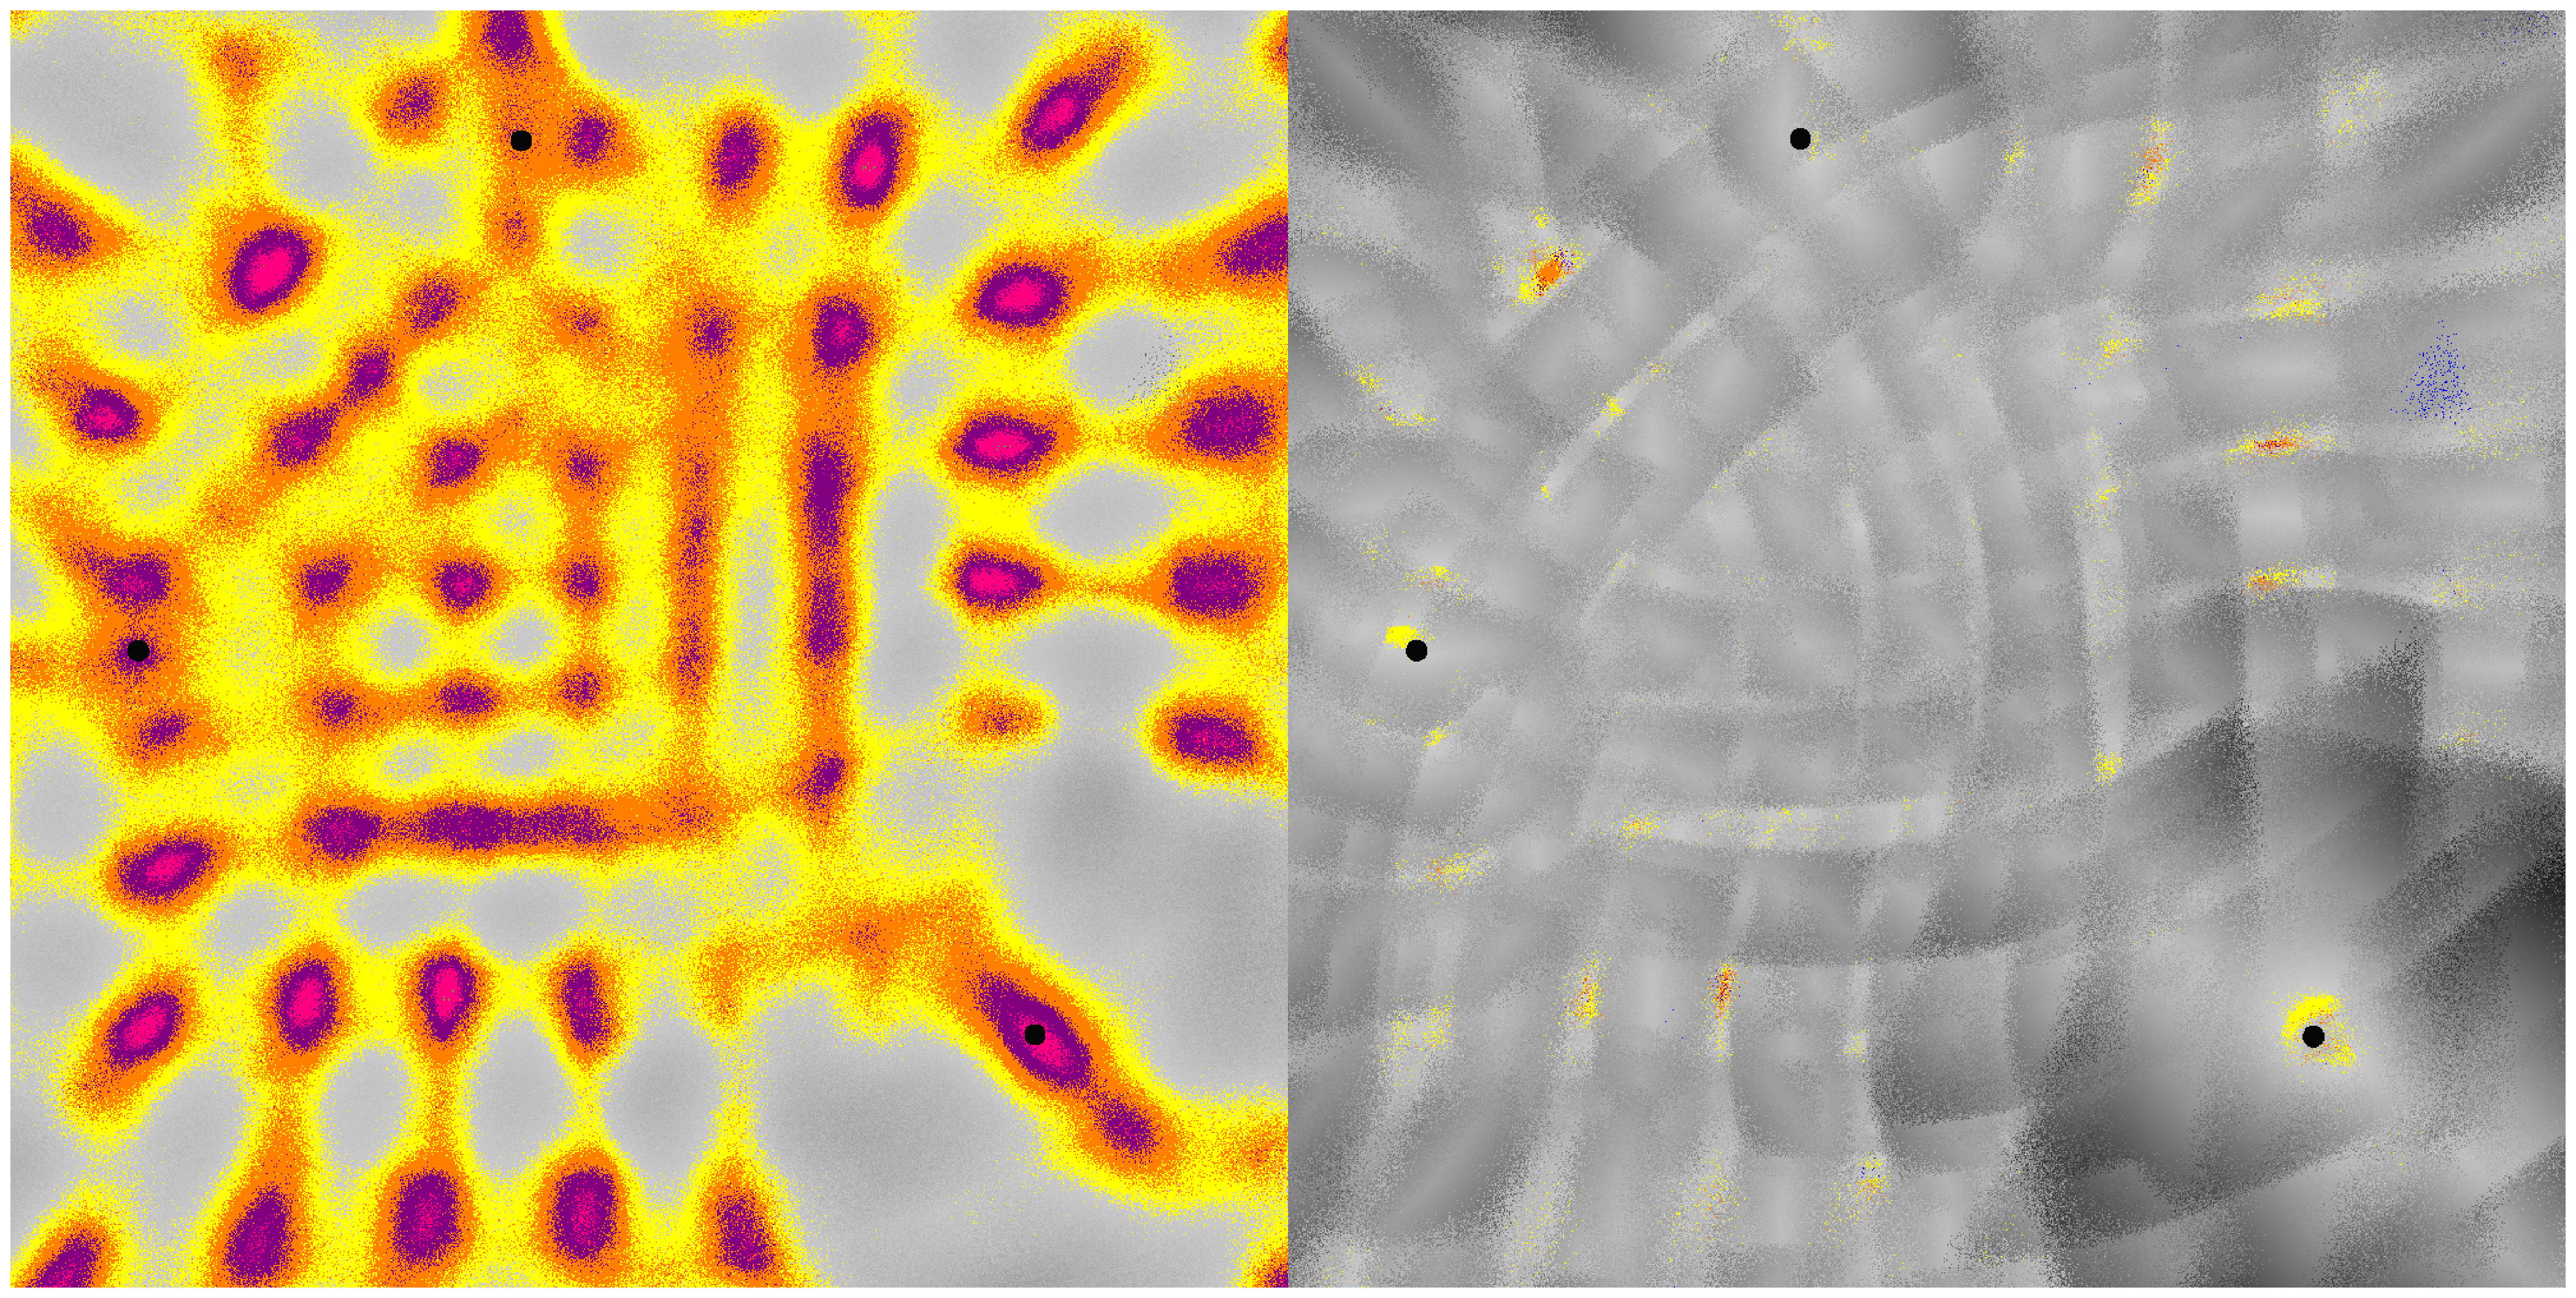
\includegraphics[width=14cm]{img/lateration}
\end{center}
\caption{Example output of the LS$^{2}$ engine}
\label{fig:lateration}
\end{figure}

The application is divided into three main parts: The engine itself, responsible for distributing the work load and calculating the position errors, a set of error models, which are used to simulate the distance measurement errors, and the lateration algorithms. Parametrized with a set of anchor positions, the error model, and the desired algorithm, the engine first starts a number of threads and associates them with a spatial slice of the 1000x1000 playing field. For each position in its slice, a thread calculates the real distance between the position and the anchors, randomly modifies the distances according to the error model, and executes the lateration algorithm. It then calculates the algorithm error as the difference between the real distance and the algorithm's return value. This process is repeated for a configurable number of iterations (defaults to 40) for each position, before the resulting average error is written back to an image buffer. At the time of writing, LS$^{2}$ features 6 different lateration algorithms, of which 4 are standard algorithms such as trilateration or \emph{Adapted Multilateration} (AML) and 2 are novel algorithms provided by the authors themselves. Regarding the error model, the user can choose between a uniform distribution and a Gaussian distribution of error values, although work is underway to support map-based error models as well.

The LS$^{2}$ engine is implemented in C99 dialect and is heavily optimized for speed. All functions are forcibly inlined and reside in the same compilation unit. Apart from the image buffer, no dynamically allocated memory is used. The engine itself uses SSE instructions or, at the user's wish, the newer AVX instructions available on Intel's most recent Sandy Bridge microprocessors, to process 4 respectivly 8 iterations at once. For example, the calculation of the true distances is fully vectorized as is the random number generator used by the error models. Afterwards, the engine will execute the user-requested lateration algorithm with vectorized parameters. To understand the mechanics, refer to listing \ref{prototype} which shows the function definition of the trilateration algorithm. The \texttt{count} parameter specifies the number of anchors the algorithm should use, whose x- and y-coordinates are contained in the \texttt{vx} and \texttt{vy} arrays. Note, that these, as well as the distance array \texttt{r} and the result buffers \texttt{resx} and \texttt{resy}, are declared as \texttt{VECTOR}s, which means that there are 4 (resp. 8) of each of these values waiting to be processed at once. Note that \texttt{VECTOR} is a preprocessor \texttt{define} mapping to \texttt{\_\_mm128} when the application is compiled in SSE mode and to \texttt{\_\_mm256} in AVX mode.

\begin{code}[caption={Prototype of the \texttt{trilaterate} function},label=prototype]
void trilaterate(const int count, const VECTOR* vx, 
                 const VECTOR* vy, const VECTOR* r, 
                 VECTOR* resx, VECTOR* resy);
\end{code}

When I started looking into optimizing the LS$^{2}$ application for this thesis, some algorithms shipped with it, for example trilateration and the \emph{Linear Least Squares} algorithm, already made use of SSE instructions to process their parameters in a single run. Yet, some others were merely literal transcriptions from a scalar implementation and were not aware of vector processing at all. These algorithms (\emph{Geolateration}, \emph{Voting Based Location Estimation}, and \emph{Adapted Multilateration}) simply unwrapped the vectors at the function head, calculated the position estimations in scalar code, and packed the results back into the result buffers at the end of the function. Therefore, these three algorithms best qualified for having a deeper look into their optimization potential.

\subsection{Development approach}
During the development period, it quickly became clear to me that software optimization is not an utterly straightforward task, but instead is a rather non-linear process involving mostly trial and error methods. Quite often attempting to optimize a particular piece of code using a specific optimization technique would not lead to any performance gains, even though in theory it may have looked like a very promising measure. Yet sometimes, these attempts that seemed to be "dead-ends" at first try later became valuable complements to other optimization efforts. As a consequence, my "development process", which was anything but well-defined at the beginning, turned out to be slightly different from regular iterative processes. As it is mainly a report on my personal experiences, the following section should not be misinterpreted as a universal guideline. The described steps and tools simply suited my needs best, but may seem completely pointless for others.

\subsubsection{Determining bottlenecks through profiling}
As Donald E. Knuth has already stated memorably in 1974, it is a good idea to first determine the most performance-critical part of a piece of code before beginning with optimization work, as this is likely the only part where optimization really is worth the effort. To find that critical part, the performance bottleneck, profiling a software can be helpful. For C/C++ code and Unix-like platforms, a tool called \emph{Valgrind}\footnote{\url{http://valgrind.org}, last accessed: \today{}} has become the de-facto standard profiler utility. The Valgrind suite consists of a variety of specialized profiling tools, each of them named differently, as for instance a memory usage analyzer (Mmemcheck) that especially helps finding memory leaks, a heap profiler (Massif) for dynamic memory profiling, and a cache profiler (Cachegrind) that simulates cache utilizitation to detect cache misses. The latter is especially valuable for optimization, as it additionally counts the executed instructions for each code line and is able to estimate the amount of clock cycles the processor needs to execute them. On top of that, Cachegrind features a special option (\texttt{--branch-sim=yes}) that counts branch mispredictions and thus can identify particularly unpredictable branches. Cachegrind's result can be best viewed using the \emph{KCachegrind}\footnote{\url{http://kcachegrind.sourceforge.net/html/Home.html}, last accessed: \today{}} front-end, as demonstrated by the screenshot in figure \ref{fig:kcachegrind}.
\begin{figure}[h]
\begin{center}
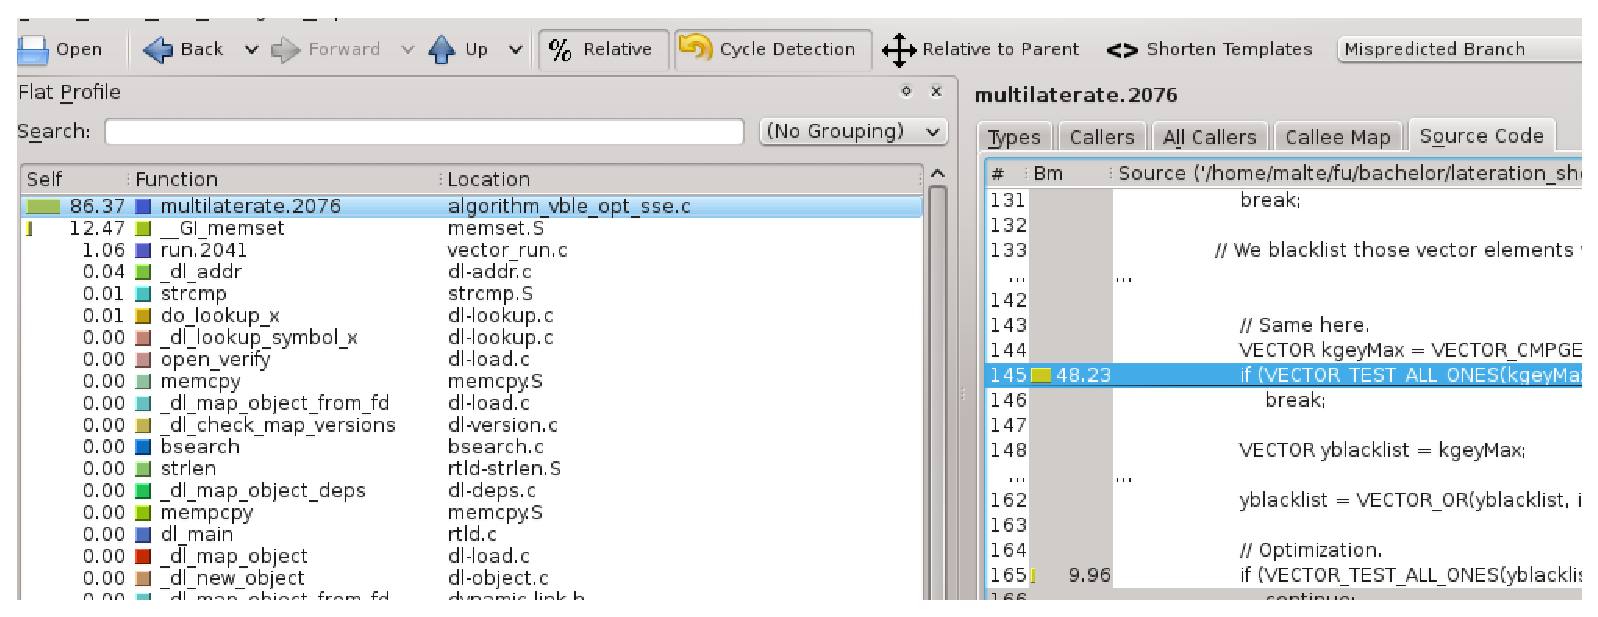
\includegraphics[width=14cm]{img/kcachegrind}
\end{center}
\caption{KCachegrind, branch prediction view}
\label{fig:kcachegrind}
\end{figure}

\subsubsection{Benchmarking optimization efforts}
After having identified the bottlenecks and resolved them with the help of optimization techniques, the next step is to evaluate their impact on performance. Before and after every smaller step, I used the unix \texttt{time} command to measure performance of the application for a randomly selected set of input values. As can be read on the command's manpage, \texttt{time} measures three different execution times, see listing \ref{time} for an example output. The "user" value indicates the amount of CPU time spent in user-mode, the "sys" value is the amount of CPU time spent in kernel-mode. The "real" value is the real time that has elapsed between start and termination of the application. For threaded applications such as LS$^{2}$, on dual-core systems this should ideally be about half of the combined "user" and "sys" times plus some overhead for context switches. As the "real" time varies with the number of processors available and the number of system-calls contained in LS$^{2}$ is close to zero, the only information that made a difference for my optimization work was the "user" value.

\begin{shell}[caption={Example output of the unix \texttt{time} command},label=time]
$ time { ./bin/lateration_shooter_sse 100 400 500 200 700 800 ; }
Average error is 45.252751

real    0m8.056s
user    0m14.916s
sys     0m0.008s
\end{shell}

As the performance of the various algorithms in LS$^{2}$ turned out to be highly affected by the positions of the anchors, it was also crucial to evaluate the performance gains using a larger amount of randomized input data, in order to avoid optimizing the application for a single case. For this time-consuming task I wrote an increasingly useful Python script dubbed \emph{benchlat}, which compiled my various work states, executed and timed them a ĺarger number of times overnight, and after completion sent me an email containing the analyzed results, namely average and variance of the runtimes. Later I added automatic profiling using Cachegrind as well as an option that allowed tracing the performance fluctuation through the development history. Regarding the selection of anchor positions, I decided to mainly choose points close to (distinct) borders of the playing field. This reduces the bias towards small, centered shapes that would arise from a uniform distribution of points and in general can be considered more realistic for localization scenarios [THIS SCREAMS CITATION.]. In order to provide statistically reliable data, benchlat empirically detected the convergence of the runtime average (after an initial threshold of 100 runs), with the convergence criterion defined as, "average has not oscillated more than $\pm0.001$s within the last 10 runs". All benchmark results displayed in the following sections have been produced by benchlat.

\subsubsection{Managing various attempts using a version control system}
As mentioned before, optimizing LS$^{2}$ was an unsteady task that was characterized by hours of trial and error. When an optimization proved to be the best solution in the very situation and to measurably improve performance, I integrated it into the sources and moved on to the next chokepoint. These successes were often preceded by a number of less profitable attempts that I wanted to save for possible later reuse. Making heavy use of lightweight branches as provided by most modern version control systems such as Git\footnote{\url{http://git-scm.com/}, last accessed: \today{}} proved highly beneficial for these cases. Using branches, I could temporarily put unpromising changes aside and merge them back in when they again seemed attractive solutions in combination with other work. To illustrate the trial and error process more vividly, figure \ref{fig:branchtree} displays a schematic overview of the development in form of a visualization of the complete Git history. Nodes represent the numerous Git commits, which are linked by arrows indicating an "ancestor-of" relationship. As can be seen easily, the development path was by no means a straightforward one.

\begin{figure}[h]
\begin{center}
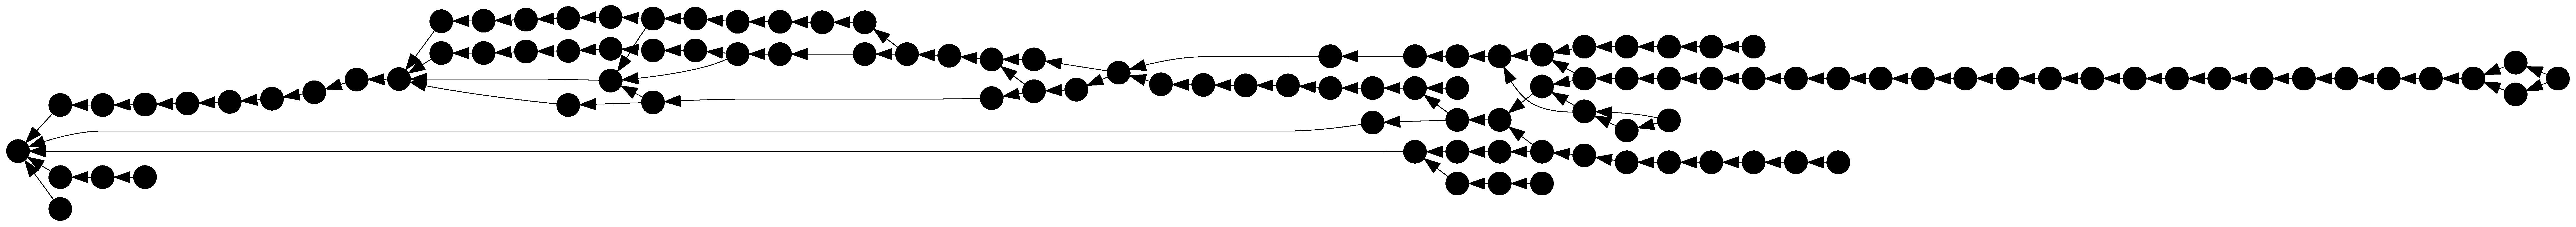
\includegraphics[width=14cm]{img/branchtree}
\end{center}
\caption{Visualization of \texttt{git} history}
\label{fig:branchtree}
\end{figure}

\subsection{Algorithm I: Adapted Multilateration}
Proposed by Kuruoglu et al. in~\cite{kuruoglu2009aml}, Adapted Multilateration (AML) is a lateration algorithm that produces acceptable results while being of lower complexity. Like in the case of tri- and multilateration, it is based on anchor circles and their intersections.

\subsubsection{Functionality}
AML consists of three steps: \emph{intersection and elimination}, \emph{first estimation}, and \emph{refinement}. At the beginning of step 1, two intersecting anchor circles are chosen randomly. If these circles intersect at exactly one point, that point is picked for step 2. In case of two circle intersections, one of them needs to be eliminated, which is the one that has the larger distance to the circle of a third anchor. Afterwards, a first estimation of the position is obtained by moving the intersection point to the middle of the line segment connecting it with the third anchor's circle (i.e. with the closest point on that circle). 
Any remaining anchors are processed in the same way in the final refinement step: For each anchor, the current location estimation is moved to the middle of the shortest line segment connecting it with the anchor's circle. Refer to the paper for a much better and more graphical explanation of the algorithm.

To calculate the said movement, the authors state it would be necessary to differentiate whether the current point is located on the inside or on the outside of the anchor's circle and treat these cases differently. However, I could not spot any reason why this method would be advantageous over using simple vector mathematics\footnote{Let $\vec{p}$ be the vector belonging to the intersection point and $\vec{x}$ the vector pointing at the center of the circle (see figure 3 in~\cite[p. 264]{kuruoglu2009aml}), while $\vec{xp} = \vec{p} - \vec{x}$ is the direction vector from Point $p$ to the center point $x$. We could then determine the intersection $a$ of the line segment between $x$ and $p$ by scaling this direction vector to the circle's radius which means multiplying the vector by $\frac{r}{\left| \vec{xp} \right|}$, i.e. as a vector: $\vec{a} = \vec{x} + \frac{r}{\left| \vec{xp}\right| } \cdot \vec{xp}$. The middle of the line segment $\overline{pa}$ can be calculated as $\vec{p'} = \vec{p} + \frac{1}{2} \cdot \vec{pa} = \vec{p} + \frac{1}{2} \cdot \left( \left( \vec{x} + \frac{r}{\left|\vec{xp}\right|} \cdot \vec{xp} \right) - \vec{p} \right)$.}. Still, as algorithmic optimization was not part of my assignment, the optimized code presented in the following corresponds to the author's original algorithm description.

\subsubsection{Optimizations}
Since the AML implementation is concise and easily understood, I will be able to present it in its entirety in this section. For a more generic start, listing \ref{circles} displays the already vectorized \texttt{circle\_get\_intersections\_v} function, which, as its name implies, is used to calculate the intersections of two random anchor circles in step 1 of AML, although it is written to process 4 pairs of circles at once, or 8 in the case of AVX. For reference, I included the original scalar implementation of this function in appendix \ref{scalarcircles}. The function is based on the usual geometric approach of constructing a line through the intersections and using triangles to determine the offset of the intersections from the line segment connecting the anchors (refer to~\cite{bourke1997circles}) for further explanation). What is most interesting in the SSE implementation, is the treatment of special cases occurring when the circles do not (properly) intersect, of which there are three: First, the circles may be disjunct, i.e. the distance between the anchors is greater than the sum of the circles' radii, second, one circle may be contained within the other (the absolute difference of the radii is less than the distance between the anchors), and third, the anchors may be coincident (the distance is 0), in which case there are 0 or an infinite number of intersections. In the original implementation these special cases were handled by an \texttt{if} statement that contained three boolean expressions linked by logical OR, each of them corresponding to one of the cases. In case the \texttt{if} statement evaluated to \texttt{true}, the function would immediately return 0. To eliminate the conditional jump, the SSE version inverts the boolean expressions and blends the \texttt{retval} vector to 1 in case all expressions are true, 0 otherwise (ll. 11-13 in listing \ref{circles}). Afterwards, all the usual calculations are performed regardless of whether the circles contained in the particular vectors truly intersect, which may result in unusual values for vector elements that failed the blending before. For example, coincident anchors, having a distance of 0, will lead to a division by zero in line 15, which results in variable \texttt{a} containing the floating-point-specific value \texttt{+Inf}, or "positive infinity". In fact, all intermediary results should be considered "tainted" until they are verified by re-checking the mask that is now stored in \texttt{retval}. An example can be seen in line 33: If variable \texttt{h}, containing the distance between the intersection(s) and the line segment connecting the anchors, is non-zero, the algorithm has found two intersections. In this case, \texttt{retval} is again incremented to indicate two solutions, but only when it already holds a 1, in other words, when all special cases have been ruled out. As a noteworthy side-effect, the SSE implementation always modifies the \texttt{resx} and \texttt{resy} vectors, while the scalar implementation did not touch them if the circles did not intersect.

\codefile{Calculating circle intersections with SSE}{circles}{code/circles.c}

\subsubsection{Evaluation}

\subsection{Algorithm II: Geolateration}
\subsection{Algorithm III: Optimized Voting Based Location Estimation}
\subsection{Framework}
--> movntps yyx